\documentclass[1p]{elsarticle_modified}
%\bibliographystyle{elsarticle-num}

%\usepackage[colorlinks]{hyperref}
%\usepackage{abbrmath_seonhwa} %\Abb, \Ascr, \Acal ,\Abf, \Afrak
\usepackage{amsfonts}
\usepackage{amssymb}
\usepackage{amsmath}
\usepackage{amsthm}
\usepackage{scalefnt}
\usepackage{amsbsy}
\usepackage{kotex}
\usepackage{caption}
\usepackage{subfig}
\usepackage{color}
\usepackage{graphicx}
\usepackage{xcolor} %% white, black, red, green, blue, cyan, magenta, yellow
\usepackage{float}
\usepackage{setspace}
\usepackage{hyperref}

\usepackage{tikz}
\usetikzlibrary{arrows}

\usepackage{multirow}
\usepackage{array} % fixed length table
\usepackage{hhline}

%%%%%%%%%%%%%%%%%%%%%
\makeatletter
\renewcommand*\env@matrix[1][\arraystretch]{%
	\edef\arraystretch{#1}%
	\hskip -\arraycolsep
	\let\@ifnextchar\new@ifnextchar
	\array{*\c@MaxMatrixCols c}}
\makeatother %https://tex.stackexchange.com/questions/14071/how-can-i-increase-the-line-spacing-in-a-matrix
%%%%%%%%%%%%%%%

\usepackage[normalem]{ulem}

\newcommand{\msout}[1]{\ifmmode\text{\sout{\ensuremath{#1}}}\else\sout{#1}\fi}
%SOURCE: \msout is \stkout macro in https://tex.stackexchange.com/questions/20609/strikeout-in-math-mode

\newcommand{\cancel}[1]{
	\ifmmode
	{\color{red}\msout{#1}}
	\else
	{\color{red}\sout{#1}}
	\fi
}

\newcommand{\add}[1]{
	{\color{blue}\uwave{#1}}
}

\newcommand{\replace}[2]{
	\ifmmode
	{\color{red}\msout{#1}}{\color{blue}\uwave{#2}}
	\else
	{\color{red}\sout{#1}}{\color{blue}\uwave{#2}}
	\fi
}

\newcommand{\Sol}{\mathcal{S}} %segment
\newcommand{\D}{D} %diagram
\newcommand{\A}{\mathcal{A}} %arc


%%%%%%%%%%%%%%%%%%%%%%%%%%%%%5 test

\def\sl{\operatorname{\textup{SL}}(2,\Cbb)}
\def\psl{\operatorname{\textup{PSL}}(2,\Cbb)}
\def\quan{\mkern 1mu \triangleright \mkern 1mu}

\theoremstyle{definition}
\newtheorem{thm}{Theorem}[section]
\newtheorem{prop}[thm]{Proposition}
\newtheorem{lem}[thm]{Lemma}
\newtheorem{ques}[thm]{Question}
\newtheorem{cor}[thm]{Corollary}
\newtheorem{defn}[thm]{Definition}
\newtheorem{exam}[thm]{Example}
\newtheorem{rmk}[thm]{Remark}
\newtheorem{alg}[thm]{Algorithm}

\newcommand{\I}{\sqrt{-1}}
\begin{document}

%\begin{frontmatter}
%
%\title{Boundary parabolic representations of knots up to 8 crossings}
%
%%% Group authors per affiliation:
%\author{Yunhi Cho} 
%\address{Department of Mathematics, University of Seoul, Seoul, Korea}
%\ead{yhcho@uos.ac.kr}
%
%
%\author{Seonhwa Kim} %\fnref{s_kim}}
%\address{Center for Geometry and Physics, Institute for Basic Science, Pohang, 37673, Korea}
%\ead{ryeona17@ibs.re.kr}
%
%\author{Hyuk Kim}
%\address{Department of Mathematical Sciences, Seoul National University, Seoul 08826, Korea}
%\ead{hyukkim@snu.ac.kr}
%
%\author{Seokbeom Yoon}
%\address{Department of Mathematical Sciences, Seoul National University, Seoul, 08826,  Korea}
%\ead{sbyoon15@snu.ac.kr}
%
%\begin{abstract}
%We find all boundary parabolic representation of knots up to 8 crossings.
%
%\end{abstract}
%\begin{keyword}
%    \MSC[2010] 57M25 
%\end{keyword}
%
%\end{frontmatter}

%\linenumbers
%\tableofcontents
%
\newcommand\colored[1]{\textcolor{white}{\rule[-0.35ex]{0.8em}{1.4ex}}\kern-0.8em\color{red} #1}%
%\newcommand\colored[1]{\textcolor{white}{ #1}\kern-2.17ex	\textcolor{white}{ #1}\kern-1.81ex	\textcolor{white}{ #1}\kern-2.15ex\color{red}#1	}

{\Large $\underline{12n_{0593}~(K12n_{0593})}$}

\setlength{\tabcolsep}{10pt}
\renewcommand{\arraystretch}{1.6}
\vspace{1cm}\begin{tabular}{m{100pt}>{\centering\arraybackslash}m{274pt}}
\multirow{5}{120pt}{
	\centering
	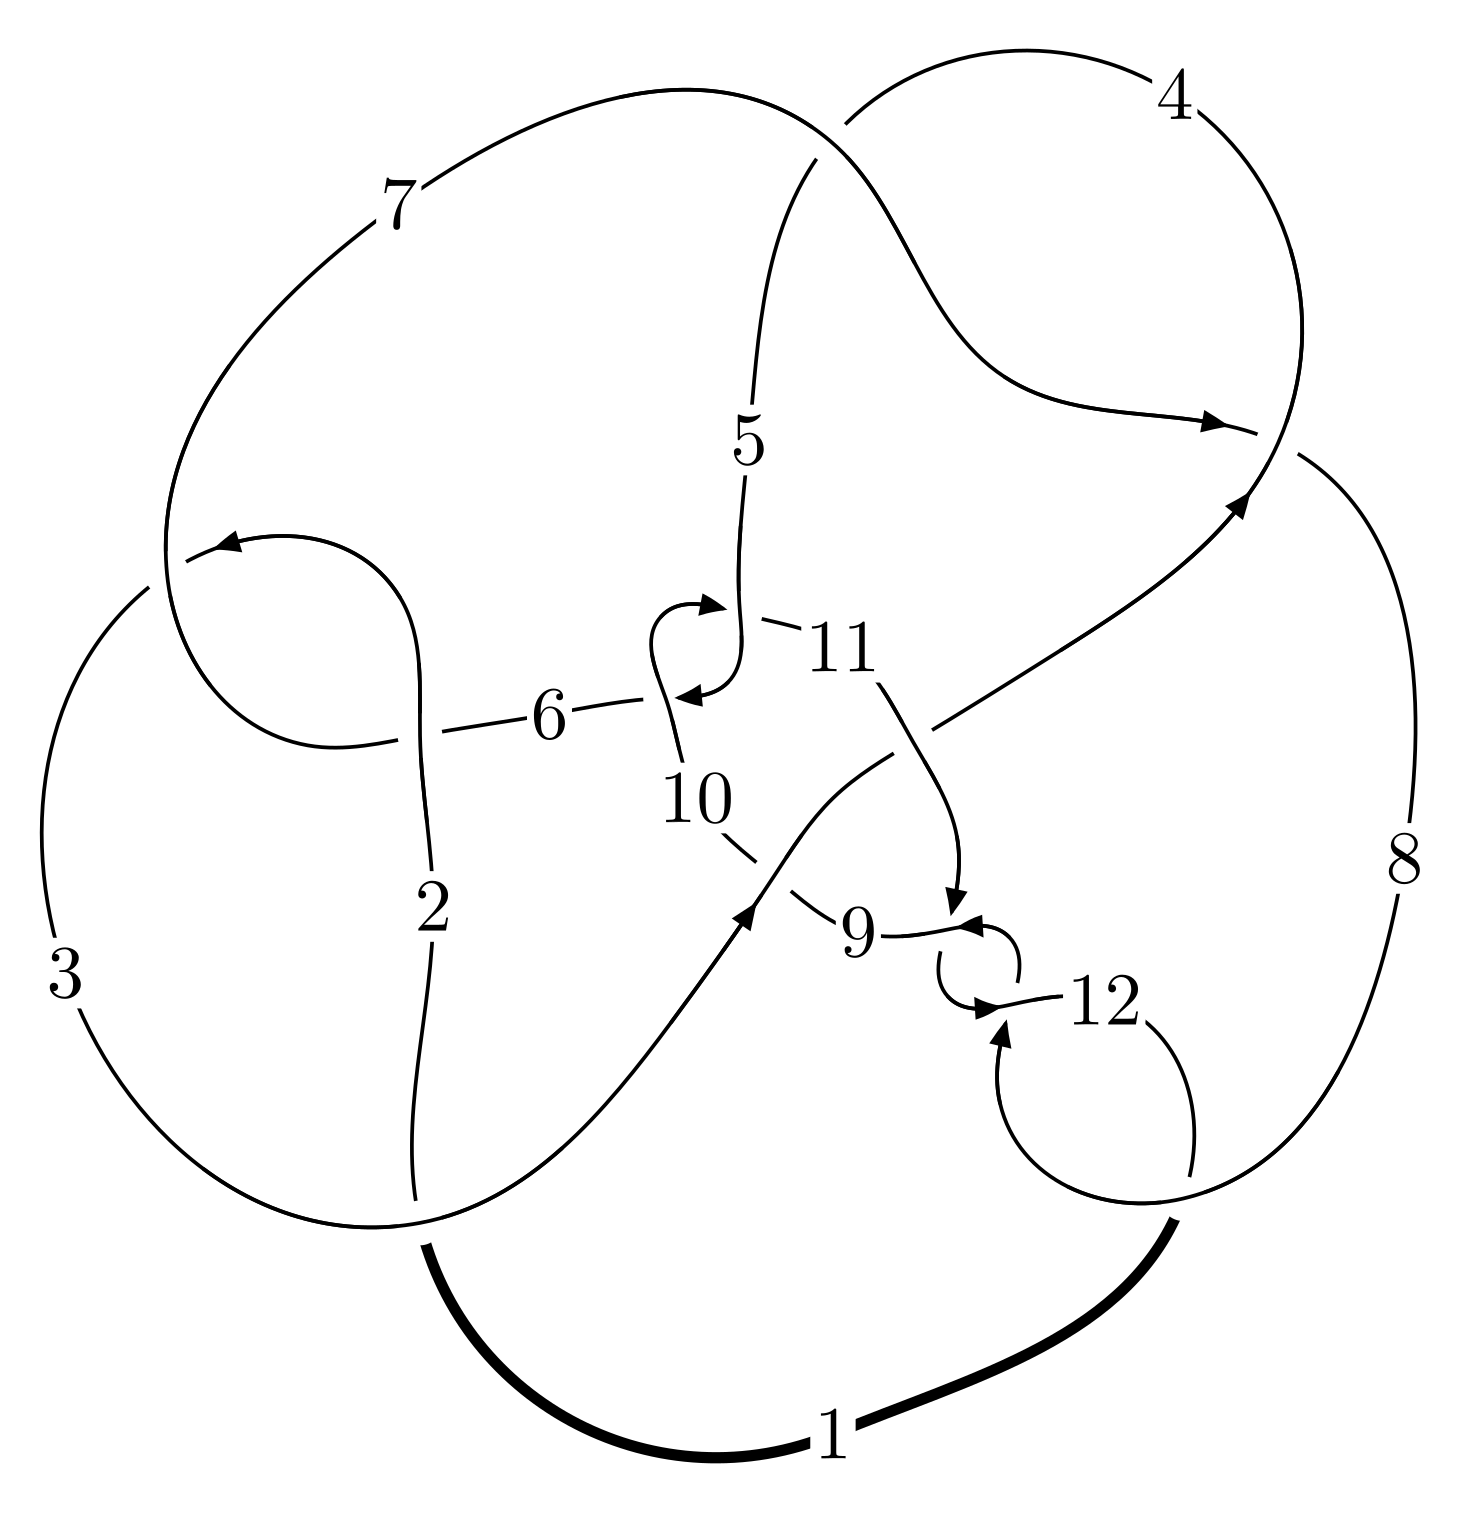
\includegraphics[width=112pt]{../../../GIT/diagram.site/Diagrams/png/2682_12n_0593.png}\\
\ \ \ A knot diagram\footnotemark}&
\allowdisplaybreaks
\textbf{Linearized knot diagam} \\
\cline{2-2}
 &
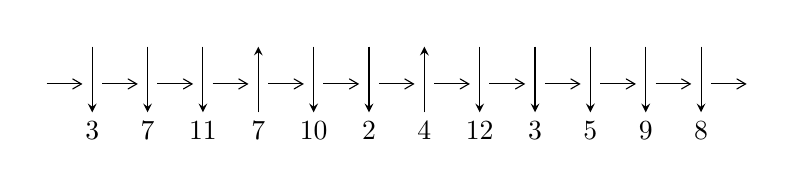
\begin{tikzpicture}[x=20pt, y=17pt]
	% nodes
	\node (C0) at (0, 0) {};
	\node (C1) at (1, 0) {};
	\node (C1U) at (1, +1) {};
	\node (C1D) at (1, -1) {3};

	\node (C2) at (2, 0) {};
	\node (C2U) at (2, +1) {};
	\node (C2D) at (2, -1) {7};

	\node (C3) at (3, 0) {};
	\node (C3U) at (3, +1) {};
	\node (C3D) at (3, -1) {11};

	\node (C4) at (4, 0) {};
	\node (C4U) at (4, +1) {};
	\node (C4D) at (4, -1) {7};

	\node (C5) at (5, 0) {};
	\node (C5U) at (5, +1) {};
	\node (C5D) at (5, -1) {10};

	\node (C6) at (6, 0) {};
	\node (C6U) at (6, +1) {};
	\node (C6D) at (6, -1) {2};

	\node (C7) at (7, 0) {};
	\node (C7U) at (7, +1) {};
	\node (C7D) at (7, -1) {4};

	\node (C8) at (8, 0) {};
	\node (C8U) at (8, +1) {};
	\node (C8D) at (8, -1) {12};

	\node (C9) at (9, 0) {};
	\node (C9U) at (9, +1) {};
	\node (C9D) at (9, -1) {3};

	\node (C10) at (10, 0) {};
	\node (C10U) at (10, +1) {};
	\node (C10D) at (10, -1) {5};

	\node (C11) at (11, 0) {};
	\node (C11U) at (11, +1) {};
	\node (C11D) at (11, -1) {9};

	\node (C12) at (12, 0) {};
	\node (C12U) at (12, +1) {};
	\node (C12D) at (12, -1) {8};
	\node (C13) at (13, 0) {};

	% arrows
	\draw[->,>={angle 60}]
	(C0) edge (C1) (C1) edge (C2) (C2) edge (C3) (C3) edge (C4) (C4) edge (C5) (C5) edge (C6) (C6) edge (C7) (C7) edge (C8) (C8) edge (C9) (C9) edge (C10) (C10) edge (C11) (C11) edge (C12) (C12) edge (C13) ;	\draw[->,>=stealth]
	(C1U) edge (C1D) (C2U) edge (C2D) (C3U) edge (C3D) (C4D) edge (C4U) (C5U) edge (C5D) (C6U) edge (C6D) (C7D) edge (C7U) (C8U) edge (C8D) (C9U) edge (C9D) (C10U) edge (C10D) (C11U) edge (C11D) (C12U) edge (C12D) ;
	\end{tikzpicture} \\
\hhline{~~} \\& 
\textbf{Solving Sequence} \\ \cline{2-2} 
 &
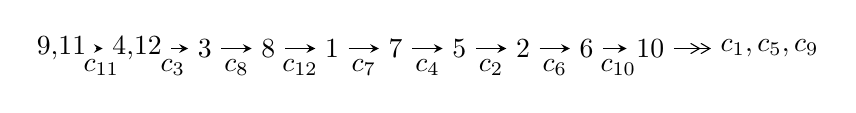
\begin{tikzpicture}[x=23pt, y=7pt]
	% node
	\node (A0) at (-1/8, 0) {9,11};
	\node (A1) at (17/16, 0) {4,12};
	\node (A2) at (17/8, 0) {3};
	\node (A3) at (25/8, 0) {8};
	\node (A4) at (33/8, 0) {1};
	\node (A5) at (41/8, 0) {7};
	\node (A6) at (49/8, 0) {5};
	\node (A7) at (57/8, 0) {2};
	\node (A8) at (65/8, 0) {6};
	\node (A9) at (73/8, 0) {10};
	\node (C1) at (1/2, -1) {$c_{11}$};
	\node (C2) at (13/8, -1) {$c_{3}$};
	\node (C3) at (21/8, -1) {$c_{8}$};
	\node (C4) at (29/8, -1) {$c_{12}$};
	\node (C5) at (37/8, -1) {$c_{7}$};
	\node (C6) at (45/8, -1) {$c_{4}$};
	\node (C7) at (53/8, -1) {$c_{2}$};
	\node (C8) at (61/8, -1) {$c_{6}$};
	\node (C9) at (69/8, -1) {$c_{10}$};
	\node (A10) at (11, 0) {$c_{1},c_{5},c_{9}$};

	% edge
	\draw[->,>=stealth]	
	(A0) edge (A1) (A1) edge (A2) (A2) edge (A3) (A3) edge (A4) (A4) edge (A5) (A5) edge (A6) (A6) edge (A7) (A7) edge (A8) (A8) edge (A9) ;
	\draw[->>,>={angle 60}]	
	(A9) edge (A10);
\end{tikzpicture} \\ 

\end{tabular} \\

\footnotetext{
The image of knot diagram is generated by the software ``\textbf{Draw programme}" developed by Andrew Bartholomew(\url{http://www.layer8.co.uk/maths/draw/index.htm\#Running-draw}), where we modified some parts for our purpose(\url{https://github.com/CATsTAILs/LinksPainter}).
}\phantom \\ \newline 
\centering \textbf{Ideals for irreducible components\footnotemark of $X_{\text{par}}$} 
 
\begin{align*}
I^u_{1}&=\langle 
-3.56874\times10^{31} u^{44}+1.26158\times10^{34} u^{43}+\cdots+1.98880\times10^{34} b-6.49981\times10^{34},\\
\phantom{I^u_{1}}&\phantom{= \langle  }-7.56930\times10^{33} u^{44}-2.14961\times10^{35} u^{43}+\cdots+1.39216\times10^{35} a+1.06952\times10^{36},\\
\phantom{I^u_{1}}&\phantom{= \langle  }u^{45}+18 u^{43}+\cdots+19 u-7\rangle \\
I^u_{2}&=\langle 
u^{13}+u^{12}+6 u^{11}+5 u^{10}+12 u^9+8 u^8+6 u^7+3 u^6-7 u^5-2 u^4-5 u^3- u^2+b+2 u,\\
\phantom{I^u_{2}}&\phantom{= \langle  }-2 u^{14}-2 u^{13}-14 u^{12}-11 u^{11}-36 u^{10}-21 u^9-37 u^8-15 u^7-4 u^6-5 u^5+14 u^4-7 u^3+4 u^2+a-4 u,\\
\phantom{I^u_{2}}&\phantom{= \langle  }u^{15}+u^{14}+8 u^{13}+7 u^{12}+25 u^{11}+19 u^{10}+36 u^9+24 u^8+18 u^7+13 u^6-8 u^5+2 u^4-7 u^3+u^2+2 u+1\rangle \\
\\
\end{align*}
\raggedright * 2 irreducible components of $\dim_{\mathbb{C}}=0$, with total 60 representations.\\
\footnotetext{All coefficients of polynomials are rational numbers. But the coefficients are sometimes approximated in decimal forms when there is not enough margin.}
\newpage
\renewcommand{\arraystretch}{1}
\centering \section*{I. $I^u_{1}= \langle -3.57\times10^{31} u^{44}+1.26\times10^{34} u^{43}+\cdots+1.99\times10^{34} b-6.50\times10^{34},\;-7.57\times10^{33} u^{44}-2.15\times10^{35} u^{43}+\cdots+1.39\times10^{35} a+1.07\times10^{36},\;u^{45}+18 u^{43}+\cdots+19 u-7 \rangle$}
\flushleft \textbf{(i) Arc colorings}\\
\begin{tabular}{m{7pt} m{180pt} m{7pt} m{180pt} }
\flushright $a_{9}=$&$\begin{pmatrix}0\\u\end{pmatrix}$ \\
\flushright $a_{11}=$&$\begin{pmatrix}1\\0\end{pmatrix}$ \\
\flushright $a_{4}=$&$\begin{pmatrix}0.0543710 u^{44}+1.54408 u^{43}+\cdots+25.1156 u-7.68247\\0.00179442 u^{44}-0.634340 u^{43}+\cdots-9.30054 u+3.26821\end{pmatrix}$ \\
\flushright $a_{12}=$&$\begin{pmatrix}1\\u^2\end{pmatrix}$ \\
\flushright $a_{3}=$&$\begin{pmatrix}0.0561654 u^{44}+0.909740 u^{43}+\cdots+15.8151 u-4.41426\\0.00179442 u^{44}-0.634340 u^{43}+\cdots-9.30054 u+3.26821\end{pmatrix}$ \\
\flushright $a_{8}=$&$\begin{pmatrix}u\\u^3+u\end{pmatrix}$ \\
\flushright $a_{1}=$&$\begin{pmatrix}u^2+1\\u^4+2 u^2\end{pmatrix}$ \\
\flushright $a_{7}=$&$\begin{pmatrix}0.358819 u^{44}-0.964669 u^{43}+\cdots-26.2905 u+8.77144\\-0.420878 u^{44}+0.770220 u^{43}+\cdots+18.2959 u-5.48848\end{pmatrix}$ \\
\flushright $a_{5}=$&$\begin{pmatrix}0.0890726 u^{44}+2.49598 u^{43}+\cdots+43.3584 u-17.2410\\0.753177 u^{44}-0.733270 u^{43}+\cdots-18.9174 u+5.28417\end{pmatrix}$ \\
\flushright $a_{2}=$&$\begin{pmatrix}-1.09866 u^{44}+3.02308 u^{43}+\cdots+57.4402 u-18.2187\\0.664157 u^{44}-0.175210 u^{43}+\cdots-7.32914 u+0.757240\end{pmatrix}$ \\
\flushright $a_{6}=$&$\begin{pmatrix}-1.21775 u^{44}+2.63075 u^{43}+\cdots+45.0187 u-14.3526\\1.28859 u^{44}-0.261761 u^{43}+\cdots-11.5685 u+2.33427\end{pmatrix}$ \\
\flushright $a_{10}=$&$\begin{pmatrix}-2.87696 u^{44}-1.48285 u^{43}+\cdots-5.99600 u+8.64539\\0.352943 u^{44}+0.731911 u^{43}+\cdots+12.7349 u-5.07045\end{pmatrix}$\\&\end{tabular}
\flushleft \textbf{(ii) Obstruction class $= -1$}\\~\\
\flushleft \textbf{(iii) Cusp Shapes $= -0.911134 u^{44}+1.98306 u^{43}+\cdots+48.6124 u-24.1982$}\\~\\
\newpage\renewcommand{\arraystretch}{1}
\flushleft \textbf{(iv) u-Polynomials at the component}\newline \\
\begin{tabular}{m{50pt}|m{274pt}}
Crossings & \hspace{64pt}u-Polynomials at each crossing \\
\hline $$\begin{aligned}c_{1}\end{aligned}$$&$\begin{aligned}
&u^{45}+56 u^{44}+\cdots+603838 u+78961
\end{aligned}$\\
\hline $$\begin{aligned}c_{2},c_{6}\end{aligned}$$&$\begin{aligned}
&u^{45}-28 u^{43}+\cdots+1642 u-281
\end{aligned}$\\
\hline $$\begin{aligned}c_{3}\end{aligned}$$&$\begin{aligned}
&u^{45}+3 u^{44}+\cdots+25 u+5
\end{aligned}$\\
\hline $$\begin{aligned}c_{4},c_{7}\end{aligned}$$&$\begin{aligned}
&u^{45}+5 u^{44}+\cdots+23 u+1
\end{aligned}$\\
\hline $$\begin{aligned}c_{5},c_{10}\end{aligned}$$&$\begin{aligned}
&u^{45}- u^{44}+\cdots+383 u+77
\end{aligned}$\\
\hline $$\begin{aligned}c_{8},c_{11},c_{12}\end{aligned}$$&$\begin{aligned}
&u^{45}+18 u^{43}+\cdots+19 u-7
\end{aligned}$\\
\hline $$\begin{aligned}c_{9}\end{aligned}$$&$\begin{aligned}
&u^{45}+4 u^{44}+\cdots+14063662 u-7404196
\end{aligned}$\\
\hline
\end{tabular}\\~\\
\newpage\renewcommand{\arraystretch}{1}
\flushleft \textbf{(v) Riley Polynomials at the component}\newline \\
\begin{tabular}{m{50pt}|m{274pt}}
Crossings & \hspace{64pt}Riley Polynomials at each crossing \\
\hline $$\begin{aligned}c_{1}\end{aligned}$$&$\begin{aligned}
&y^{45}-120 y^{44}+\cdots-392839435230 y-6234839521
\end{aligned}$\\
\hline $$\begin{aligned}c_{2},c_{6}\end{aligned}$$&$\begin{aligned}
&y^{45}-56 y^{44}+\cdots+603838 y-78961
\end{aligned}$\\
\hline $$\begin{aligned}c_{3}\end{aligned}$$&$\begin{aligned}
&y^{45}- y^{44}+\cdots+595 y-25
\end{aligned}$\\
\hline $$\begin{aligned}c_{4},c_{7}\end{aligned}$$&$\begin{aligned}
&y^{45}+45 y^{44}+\cdots+173 y-1
\end{aligned}$\\
\hline $$\begin{aligned}c_{5},c_{10}\end{aligned}$$&$\begin{aligned}
&y^{45}+3 y^{44}+\cdots+136371 y-5929
\end{aligned}$\\
\hline $$\begin{aligned}c_{8},c_{11},c_{12}\end{aligned}$$&$\begin{aligned}
&y^{45}+36 y^{44}+\cdots-157 y-49
\end{aligned}$\\
\hline $$\begin{aligned}c_{9}\end{aligned}$$&$\begin{aligned}
&y^{45}-28 y^{44}+\cdots+252875184270700 y-54822118406416
\end{aligned}$\\
\hline
\end{tabular}\\~\\
\newpage\flushleft \textbf{(vi) Complex Volumes and Cusp Shapes}
$$\begin{array}{c|c|c}  
\text{Solutions to }I^u_{1}& \I (\text{vol} + \sqrt{-1}CS) & \text{Cusp shape}\\
 \hline 
\begin{aligned}
u &= \phantom{-}1.008740 + 0.105187 I \\
a &= -0.793375 + 0.421615 I \\
b &= -1.17957 - 1.05675 I\end{aligned}
 & -12.4412 - 8.8186 I & -11.24074 + 4.62166 I \\ \hline\begin{aligned}
u &= \phantom{-}1.008740 - 0.105187 I \\
a &= -0.793375 - 0.421615 I \\
b &= -1.17957 + 1.05675 I\end{aligned}
 & -12.4412 + 8.8186 I & -11.24074 - 4.62166 I \\ \hline\begin{aligned}
u &= -0.386406 + 0.901026 I \\
a &= \phantom{-}0.972143 - 0.261563 I \\
b &= -0.853990 - 0.224349 I\end{aligned}
 & -1.53875 + 2.61522 I & -10.52840 - 2.22098 I \\ \hline\begin{aligned}
u &= -0.386406 - 0.901026 I \\
a &= \phantom{-}0.972143 + 0.261563 I \\
b &= -0.853990 + 0.224349 I\end{aligned}
 & -1.53875 - 2.61522 I & -10.52840 + 2.22098 I \\ \hline\begin{aligned}
u &= -0.973608 + 0.085974 I \\
a &= -0.651872 + 0.166835 I \\
b &= -1.12732 - 1.18722 I\end{aligned}
 & -12.05690 + 0.39267 I & -11.73771 - 0.23193 I \\ \hline\begin{aligned}
u &= -0.973608 - 0.085974 I \\
a &= -0.651872 - 0.166835 I \\
b &= -1.12732 + 1.18722 I\end{aligned}
 & -12.05690 - 0.39267 I & -11.73771 + 0.23193 I \\ \hline\begin{aligned}
u &= \phantom{-}0.059330 + 1.065280 I \\
a &= \phantom{-}2.12098 - 2.58813 I \\
b &= \phantom{-}0.090245 + 1.168500 I\end{aligned}
 & \phantom{-}4.60968 - 0.45678 I & -4.72300 - 1.28970 I \\ \hline\begin{aligned}
u &= \phantom{-}0.059330 - 1.065280 I \\
a &= \phantom{-}2.12098 + 2.58813 I \\
b &= \phantom{-}0.090245 - 1.168500 I\end{aligned}
 & \phantom{-}4.60968 + 0.45678 I & -4.72300 + 1.28970 I \\ \hline\begin{aligned}
u &= \phantom{-}0.114676 + 1.068030 I \\
a &= \phantom{-}0.114025 + 0.194088 I \\
b &= \phantom{-}1.033700 + 0.324573 I\end{aligned}
 & \phantom{-}0.63009 - 3.63899 I & -6.69888 + 4.56263 I \\ \hline\begin{aligned}
u &= \phantom{-}0.114676 - 1.068030 I \\
a &= \phantom{-}0.114025 - 0.194088 I \\
b &= \phantom{-}1.033700 - 0.324573 I\end{aligned}
 & \phantom{-}0.63009 + 3.63899 I & -6.69888 - 4.56263 I\\
 \hline 
 \end{array}$$\newpage$$\begin{array}{c|c|c}  
\text{Solutions to }I^u_{1}& \I (\text{vol} + \sqrt{-1}CS) & \text{Cusp shape}\\
 \hline 
\begin{aligned}
u &= -1.07704\phantom{ +0.000000I} \\
a &= -0.250717\phantom{ +0.000000I} \\
b &= -0.595129\phantom{ +0.000000I}\end{aligned}
 & -5.84338\phantom{ +0.000000I} & -27.3640\phantom{ +0.000000I} \\ \hline\begin{aligned}
u &= -0.759699 + 0.408323 I \\
a &= \phantom{-}0.154012 + 0.433176 I \\
b &= \phantom{-}0.747946 - 0.618927 I\end{aligned}
 & -2.98722 + 1.75252 I & -12.73751 - 3.21228 I \\ \hline\begin{aligned}
u &= -0.759699 - 0.408323 I \\
a &= \phantom{-}0.154012 - 0.433176 I \\
b &= \phantom{-}0.747946 + 0.618927 I\end{aligned}
 & -2.98722 - 1.75252 I & -12.73751 + 3.21228 I \\ \hline\begin{aligned}
u &= \phantom{-}0.847403\phantom{ +0.000000I} \\
a &= -1.81130\phantom{ +0.000000I} \\
b &= -0.770728\phantom{ +0.000000I}\end{aligned}
 & -6.54062\phantom{ +0.000000I} & -18.4620\phantom{ +0.000000I} \\ \hline\begin{aligned}
u &= -0.130385 + 1.145750 I \\
a &= -0.383923 - 0.931720 I \\
b &= -0.511829 + 0.522136 I\end{aligned}
 & \phantom{-}2.58249 + 1.78836 I & -4.62276 - 3.94731 I \\ \hline\begin{aligned}
u &= -0.130385 - 1.145750 I \\
a &= -0.383923 + 0.931720 I \\
b &= -0.511829 - 0.522136 I\end{aligned}
 & \phantom{-}2.58249 - 1.78836 I & -4.62276 + 3.94731 I \\ \hline\begin{aligned}
u &= \phantom{-}0.288094 + 1.183980 I \\
a &= -0.40323 + 3.10896 I \\
b &= -0.594143 - 0.715509 I\end{aligned}
 & \phantom{-}0.14683 - 6.35148 I & -6.06536 + 8.65205 I \\ \hline\begin{aligned}
u &= \phantom{-}0.288094 - 1.183980 I \\
a &= -0.40323 - 3.10896 I \\
b &= -0.594143 + 0.715509 I\end{aligned}
 & \phantom{-}0.14683 + 6.35148 I & -6.06536 - 8.65205 I \\ \hline\begin{aligned}
u &= -0.072450 + 1.292850 I \\
a &= -1.19970 + 1.90753 I \\
b &= \phantom{-}0.303712 - 0.219752 I\end{aligned}
 & \phantom{-}3.92457 + 2.86801 I & \phantom{-0.000000 } 0. - 4.92967 I \\ \hline\begin{aligned}
u &= -0.072450 - 1.292850 I \\
a &= -1.19970 - 1.90753 I \\
b &= \phantom{-}0.303712 + 0.219752 I\end{aligned}
 & \phantom{-}3.92457 - 2.86801 I & \phantom{-0.000000 -}0. + 4.92967 I\\
 \hline 
 \end{array}$$\newpage$$\begin{array}{c|c|c}  
\text{Solutions to }I^u_{1}& \I (\text{vol} + \sqrt{-1}CS) & \text{Cusp shape}\\
 \hline 
\begin{aligned}
u &= \phantom{-}0.114422 + 1.323690 I \\
a &= \phantom{-}0.257409 - 0.903828 I \\
b &= -1.119530 + 0.548161 I\end{aligned}
 & \phantom{-}1.39290 + 0.75681 I & \phantom{-0.000000 } 0 \\ \hline\begin{aligned}
u &= \phantom{-}0.114422 - 1.323690 I \\
a &= \phantom{-}0.257409 + 0.903828 I \\
b &= -1.119530 - 0.548161 I\end{aligned}
 & \phantom{-}1.39290 - 0.75681 I & \phantom{-0.000000 } 0 \\ \hline\begin{aligned}
u &= \phantom{-}0.386963 + 1.277220 I \\
a &= \phantom{-}1.013090 - 0.512275 I \\
b &= \phantom{-}0.784008 - 0.030215 I\end{aligned}
 & -2.57080 - 4.43171 I & \phantom{-0.000000 } 0 \\ \hline\begin{aligned}
u &= \phantom{-}0.386963 - 1.277220 I \\
a &= \phantom{-}1.013090 + 0.512275 I \\
b &= \phantom{-}0.784008 + 0.030215 I\end{aligned}
 & -2.57080 + 4.43171 I & \phantom{-0.000000 } 0 \\ \hline\begin{aligned}
u &= -0.516771 + 1.244220 I \\
a &= \phantom{-}0.81944 + 1.89768 I \\
b &= \phantom{-}1.07051 - 1.15978 I\end{aligned}
 & -8.49081 + 4.89195 I & \phantom{-0.000000 } 0 \\ \hline\begin{aligned}
u &= -0.516771 - 1.244220 I \\
a &= \phantom{-}0.81944 - 1.89768 I \\
b &= \phantom{-}1.07051 + 1.15978 I\end{aligned}
 & -8.49081 - 4.89195 I & \phantom{-0.000000 } 0 \\ \hline\begin{aligned}
u &= \phantom{-}0.569830 + 1.241570 I \\
a &= -0.734691 + 0.190323 I \\
b &= \phantom{-}1.15852 - 1.01628 I\end{aligned}
 & -8.96525 + 3.25529 I & \phantom{-0.000000 } 0 \\ \hline\begin{aligned}
u &= \phantom{-}0.569830 - 1.241570 I \\
a &= -0.734691 - 0.190323 I \\
b &= \phantom{-}1.15852 + 1.01628 I\end{aligned}
 & -8.96525 - 3.25529 I & \phantom{-0.000000 } 0 \\ \hline\begin{aligned}
u &= \phantom{-}0.205740 + 1.371440 I \\
a &= -0.63512 + 1.75657 I \\
b &= -0.338407 - 1.348220 I\end{aligned}
 & \phantom{-}8.00276 - 3.83937 I & \phantom{-0.000000 } 0 \\ \hline\begin{aligned}
u &= \phantom{-}0.205740 - 1.371440 I \\
a &= -0.63512 - 1.75657 I \\
b &= -0.338407 + 1.348220 I\end{aligned}
 & \phantom{-}8.00276 + 3.83937 I & \phantom{-0.000000 } 0\\
 \hline 
 \end{array}$$\newpage$$\begin{array}{c|c|c}  
\text{Solutions to }I^u_{1}& \I (\text{vol} + \sqrt{-1}CS) & \text{Cusp shape}\\
 \hline 
\begin{aligned}
u &= -0.550103 + 1.293590 I \\
a &= \phantom{-}0.059859 + 0.501110 I \\
b &= \phantom{-}0.624990 - 0.274138 I\end{aligned}
 & -1.88022 + 5.73606 I & \phantom{-0.000000 } 0 \\ \hline\begin{aligned}
u &= -0.550103 - 1.293590 I \\
a &= \phantom{-}0.059859 - 0.501110 I \\
b &= \phantom{-}0.624990 + 0.274138 I\end{aligned}
 & -1.88022 - 5.73606 I & \phantom{-0.000000 } 0 \\ \hline\begin{aligned}
u &= \phantom{-}0.582077 + 0.106172 I \\
a &= \phantom{-}1.27394 + 1.42446 I \\
b &= \phantom{-}0.829596 - 0.667678 I\end{aligned}
 & -3.07621 + 3.07145 I & -13.51053 - 3.59920 I \\ \hline\begin{aligned}
u &= \phantom{-}0.582077 - 0.106172 I \\
a &= \phantom{-}1.27394 - 1.42446 I \\
b &= \phantom{-}0.829596 + 0.667678 I\end{aligned}
 & -3.07621 - 3.07145 I & -13.51053 + 3.59920 I \\ \hline\begin{aligned}
u &= -0.45273 + 1.36982 I \\
a &= -1.002820 - 0.419354 I \\
b &= \phantom{-}1.17560 + 1.20040 I\end{aligned}
 & -7.48754 + 5.49061 I & \phantom{-0.000000 } 0 \\ \hline\begin{aligned}
u &= -0.45273 - 1.36982 I \\
a &= -1.002820 + 0.419354 I \\
b &= \phantom{-}1.17560 - 1.20040 I\end{aligned}
 & -7.48754 - 5.49061 I & \phantom{-0.000000 } 0 \\ \hline\begin{aligned}
u &= \phantom{-}0.471958 + 0.271253 I \\
a &= \phantom{-}0.837882 + 0.291023 I \\
b &= \phantom{-}0.128615 + 1.136710 I\end{aligned}
 & \phantom{-}2.86451 - 1.30518 I & -1.84549 + 5.31752 I \\ \hline\begin{aligned}
u &= \phantom{-}0.471958 - 0.271253 I \\
a &= \phantom{-}0.837882 - 0.291023 I \\
b &= \phantom{-}0.128615 - 1.136710 I\end{aligned}
 & \phantom{-}2.86451 + 1.30518 I & -1.84549 - 5.31752 I \\ \hline\begin{aligned}
u &= \phantom{-}0.46756 + 1.38448 I \\
a &= \phantom{-}0.47175 - 1.91674 I \\
b &= \phantom{-}1.18172 + 1.08384 I\end{aligned}
 & -7.7658 - 14.0813 I & \phantom{-0.000000 } 0 \\ \hline\begin{aligned}
u &= \phantom{-}0.46756 - 1.38448 I \\
a &= \phantom{-}0.47175 + 1.91674 I \\
b &= \phantom{-}1.18172 - 1.08384 I\end{aligned}
 & -7.7658 + 14.0813 I & \phantom{-0.000000 } 0\\
 \hline 
 \end{array}$$\newpage$$\begin{array}{c|c|c}  
\text{Solutions to }I^u_{1}& \I (\text{vol} + \sqrt{-1}CS) & \text{Cusp shape}\\
 \hline 
\begin{aligned}
u &= -0.22570 + 1.49863 I \\
a &= \phantom{-}0.21030 - 1.42436 I \\
b &= -0.691548 + 0.992057 I\end{aligned}
 & \phantom{-}3.35542 + 5.28363 I & \phantom{-0.000000 } 0 \\ \hline\begin{aligned}
u &= -0.22570 - 1.49863 I \\
a &= \phantom{-}0.21030 + 1.42436 I \\
b &= -0.691548 - 0.992057 I\end{aligned}
 & \phantom{-}3.35542 - 5.28363 I & \phantom{-0.000000 } 0 \\ \hline\begin{aligned}
u &= \phantom{-}0.094137 + 0.391258 I \\
a &= \phantom{-}2.78827 - 0.14083 I \\
b &= -0.752412 + 0.154261 I\end{aligned}
 & -1.06912 + 2.39494 I & -7.24233 + 0.84783 I \\ \hline\begin{aligned}
u &= \phantom{-}0.094137 - 0.391258 I \\
a &= \phantom{-}2.78827 + 0.14083 I \\
b &= -0.752412 - 0.154261 I\end{aligned}
 & -1.06912 - 2.39494 I & -7.24233 - 0.84783 I \\ \hline\begin{aligned}
u &= -0.361714\phantom{ +0.000000I} \\
a &= \phantom{-}0.913846\phantom{ +0.000000I} \\
b &= \phantom{-}0.445021\phantom{ +0.000000I}\end{aligned}
 & -0.670926\phantom{ +0.000000I} & -14.8180\phantom{ +0.000000I}\\
 \hline 
 \end{array}$$\newpage\newpage\renewcommand{\arraystretch}{1}
\centering \section*{II. $I^u_{2}= \langle u^{13}+u^{12}+\cdots+b+2 u,\;-2 u^{14}-2 u^{13}+\cdots+a-4 u,\;u^{15}+u^{14}+\cdots+2 u+1 \rangle$}
\flushleft \textbf{(i) Arc colorings}\\
\begin{tabular}{m{7pt} m{180pt} m{7pt} m{180pt} }
\flushright $a_{9}=$&$\begin{pmatrix}0\\u\end{pmatrix}$ \\
\flushright $a_{11}=$&$\begin{pmatrix}1\\0\end{pmatrix}$ \\
\flushright $a_{4}=$&$\begin{pmatrix}2 u^{14}+2 u^{13}+\cdots-4 u^2+4 u\\- u^{13}- u^{12}+\cdots+u^2-2 u\end{pmatrix}$ \\
\flushright $a_{12}=$&$\begin{pmatrix}1\\u^2\end{pmatrix}$ \\
\flushright $a_{3}=$&$\begin{pmatrix}2 u^{14}+u^{13}+\cdots-3 u^2+2 u\\- u^{13}- u^{12}+\cdots+u^2-2 u\end{pmatrix}$ \\
\flushright $a_{8}=$&$\begin{pmatrix}u\\u^3+u\end{pmatrix}$ \\
\flushright $a_{1}=$&$\begin{pmatrix}u^2+1\\u^4+2 u^2\end{pmatrix}$ \\
\flushright $a_{7}=$&$\begin{pmatrix}u^{14}+2 u^{13}+\cdots+4 u-2\\u^{14}+u^{13}+\cdots+2 u+1\end{pmatrix}$ \\
\flushright $a_{5}=$&$\begin{pmatrix}3 u^{13}+2 u^{12}+\cdots+2 u-1\\u^{10}+u^9+5 u^8+4 u^7+8 u^6+5 u^5+3 u^4+2 u^3-2 u^2+u\end{pmatrix}$ \\
\flushright $a_{2}=$&$\begin{pmatrix}2 u^{14}+3 u^{13}+\cdots+u+2\\- u^{14}-2 u^{13}+\cdots-3 u-1\end{pmatrix}$ \\
\flushright $a_{6}=$&$\begin{pmatrix}-2 u^{14}-3 u^{13}+\cdots-2 u-2\\u^{14}+2 u^{13}+\cdots+3 u+1\end{pmatrix}$ \\
\flushright $a_{10}=$&$\begin{pmatrix}-2 u^{14}- u^{13}+\cdots+4 u+1\\- u^{13}- u^{12}-7 u^{11}-6 u^{10}-18 u^9-13 u^8-18 u^7-11 u^6-2 u^4+8 u^3\end{pmatrix}$\\&\end{tabular}
\flushleft \textbf{(ii) Obstruction class $= 1$}\\~\\
\flushleft \textbf{(iii) Cusp Shapes $= - u^{14}+u^{13}-10 u^{12}+4 u^{11}-35 u^{10}+4 u^9-50 u^8-3 u^7-11 u^6-12 u^5+36 u^4-19 u^3+18 u^2-10 u-12$}\\~\\
\newpage\renewcommand{\arraystretch}{1}
\flushleft \textbf{(iv) u-Polynomials at the component}\newline \\
\begin{tabular}{m{50pt}|m{274pt}}
Crossings & \hspace{64pt}u-Polynomials at each crossing \\
\hline $$\begin{aligned}c_{1}\end{aligned}$$&$\begin{aligned}
&u^{15}-13 u^{14}+\cdots+9 u-1
\end{aligned}$\\
\hline $$\begin{aligned}c_{2}\end{aligned}$$&$\begin{aligned}
&u^{15}- u^{14}+\cdots+3 u-1
\end{aligned}$\\
\hline $$\begin{aligned}c_{3}\end{aligned}$$&$\begin{aligned}
&u^{15}-2 u^{14}+\cdots+5 u^2-1
\end{aligned}$\\
\hline $$\begin{aligned}c_{4}\end{aligned}$$&$\begin{aligned}
&u^{15}+2 u^{14}+\cdots-4 u^2-1
\end{aligned}$\\
\hline $$\begin{aligned}c_{5}\end{aligned}$$&$\begin{aligned}
&u^{15}+7 u^{13}+\cdots+3 u^2+1
\end{aligned}$\\
\hline $$\begin{aligned}c_{6}\end{aligned}$$&$\begin{aligned}
&u^{15}+u^{14}+\cdots+3 u+1
\end{aligned}$\\
\hline $$\begin{aligned}c_{7}\end{aligned}$$&$\begin{aligned}
&u^{15}-2 u^{14}+\cdots+4 u^2+1
\end{aligned}$\\
\hline $$\begin{aligned}c_{8}\end{aligned}$$&$\begin{aligned}
&u^{15}- u^{14}+\cdots+2 u-1
\end{aligned}$\\
\hline $$\begin{aligned}c_{9}\end{aligned}$$&$\begin{aligned}
&u^{15}+5 u^{14}+\cdots-10 u+52
\end{aligned}$\\
\hline $$\begin{aligned}c_{10}\end{aligned}$$&$\begin{aligned}
&u^{15}+7 u^{13}+\cdots-3 u^2-1
\end{aligned}$\\
\hline $$\begin{aligned}c_{11},c_{12}\end{aligned}$$&$\begin{aligned}
&u^{15}+u^{14}+\cdots+2 u+1
\end{aligned}$\\
\hline
\end{tabular}\\~\\
\newpage\renewcommand{\arraystretch}{1}
\flushleft \textbf{(v) Riley Polynomials at the component}\newline \\
\begin{tabular}{m{50pt}|m{274pt}}
Crossings & \hspace{64pt}Riley Polynomials at each crossing \\
\hline $$\begin{aligned}c_{1}\end{aligned}$$&$\begin{aligned}
&y^{15}-9 y^{14}+\cdots-7 y-1
\end{aligned}$\\
\hline $$\begin{aligned}c_{2},c_{6}\end{aligned}$$&$\begin{aligned}
&y^{15}-13 y^{14}+\cdots+9 y-1
\end{aligned}$\\
\hline $$\begin{aligned}c_{3}\end{aligned}$$&$\begin{aligned}
&y^{15}+6 y^{14}+\cdots+10 y-1
\end{aligned}$\\
\hline $$\begin{aligned}c_{4},c_{7}\end{aligned}$$&$\begin{aligned}
&y^{15}+8 y^{14}+\cdots-8 y-1
\end{aligned}$\\
\hline $$\begin{aligned}c_{5},c_{10}\end{aligned}$$&$\begin{aligned}
&y^{15}+14 y^{14}+\cdots-6 y-1
\end{aligned}$\\
\hline $$\begin{aligned}c_{8},c_{11},c_{12}\end{aligned}$$&$\begin{aligned}
&y^{15}+15 y^{14}+\cdots+2 y-1
\end{aligned}$\\
\hline $$\begin{aligned}c_{9}\end{aligned}$$&$\begin{aligned}
&y^{15}+7 y^{14}+\cdots-5828 y-2704
\end{aligned}$\\
\hline
\end{tabular}\\~\\
\newpage\flushleft \textbf{(vi) Complex Volumes and Cusp Shapes}
$$\begin{array}{c|c|c}  
\text{Solutions to }I^u_{2}& \I (\text{vol} + \sqrt{-1}CS) & \text{Cusp shape}\\
 \hline 
\begin{aligned}
u &= -0.957819\phantom{ +0.000000I} \\
a &= -0.661926\phantom{ +0.000000I} \\
b &= -0.464046\phantom{ +0.000000I}\end{aligned}
 & -5.43240\phantom{ +0.000000I} & -5.96330\phantom{ +0.000000I} \\ \hline\begin{aligned}
u &= \phantom{-}0.170684 + 1.191940 I \\
a &= \phantom{-}1.99278 - 2.50947 I \\
b &= -0.224051 + 0.994213 I\end{aligned}
 & \phantom{-}4.95411 - 1.54403 I & -1.95869 + 3.90888 I \\ \hline\begin{aligned}
u &= \phantom{-}0.170684 - 1.191940 I \\
a &= \phantom{-}1.99278 + 2.50947 I \\
b &= -0.224051 - 0.994213 I\end{aligned}
 & \phantom{-}4.95411 + 1.54403 I & -1.95869 - 3.90888 I \\ \hline\begin{aligned}
u &= -0.065754 + 1.280360 I \\
a &= -0.214962 + 0.173404 I \\
b &= -1.132550 - 0.235968 I\end{aligned}
 & \phantom{-}2.00576 - 2.03853 I & -5.38866 + 3.46155 I \\ \hline\begin{aligned}
u &= -0.065754 - 1.280360 I \\
a &= -0.214962 - 0.173404 I \\
b &= -1.132550 + 0.235968 I\end{aligned}
 & \phantom{-}2.00576 + 2.03853 I & -5.38866 - 3.46155 I \\ \hline\begin{aligned}
u &= -0.438447 + 1.226120 I \\
a &= \phantom{-}0.397262 - 0.091676 I \\
b &= \phantom{-}0.546264 - 0.057068 I\end{aligned}
 & -1.69926 + 4.99019 I & -7.83136 - 3.68033 I \\ \hline\begin{aligned}
u &= -0.438447 - 1.226120 I \\
a &= \phantom{-}0.397262 + 0.091676 I \\
b &= \phantom{-}0.546264 + 0.057068 I\end{aligned}
 & -1.69926 - 4.99019 I & -7.83136 + 3.68033 I \\ \hline\begin{aligned}
u &= \phantom{-}0.574249 + 0.201778 I \\
a &= -0.090007 + 0.468927 I \\
b &= \phantom{-}0.257595 + 1.314620 I\end{aligned}
 & \phantom{-}2.04734 - 1.06098 I & -12.25326 + 1.45022 I \\ \hline\begin{aligned}
u &= \phantom{-}0.574249 - 0.201778 I \\
a &= -0.090007 - 0.468927 I \\
b &= \phantom{-}0.257595 - 1.314620 I\end{aligned}
 & \phantom{-}2.04734 + 1.06098 I & -12.25326 - 1.45022 I \\ \hline\begin{aligned}
u &= \phantom{-}0.227689 + 1.394080 I \\
a &= -0.46823 + 1.79191 I \\
b &= -0.35742 - 1.57983 I\end{aligned}
 & \phantom{-}7.19370 - 4.01988 I & -7.47475 + 4.21701 I\\
 \hline 
 \end{array}$$\newpage$$\begin{array}{c|c|c}  
\text{Solutions to }I^u_{2}& \I (\text{vol} + \sqrt{-1}CS) & \text{Cusp shape}\\
 \hline 
\begin{aligned}
u &= \phantom{-}0.227689 - 1.394080 I \\
a &= -0.46823 - 1.79191 I \\
b &= -0.35742 + 1.57983 I\end{aligned}
 & \phantom{-}7.19370 + 4.01988 I & -7.47475 - 4.21701 I \\ \hline\begin{aligned}
u &= -0.17862 + 1.44151 I \\
a &= \phantom{-}0.40873 - 1.60438 I \\
b &= -0.707302 + 0.825528 I\end{aligned}
 & \phantom{-}4.37895 + 5.24684 I & -1.49909 - 5.49903 I \\ \hline\begin{aligned}
u &= -0.17862 - 1.44151 I \\
a &= \phantom{-}0.40873 + 1.60438 I \\
b &= -0.707302 - 0.825528 I\end{aligned}
 & \phantom{-}4.37895 - 5.24684 I & -1.49909 + 5.49903 I \\ \hline\begin{aligned}
u &= -0.310890 + 0.262705 I \\
a &= -0.69461 + 2.22045 I \\
b &= \phantom{-}0.849487 - 0.449404 I\end{aligned}
 & -1.36000 + 3.17848 I & -10.11254 - 7.00555 I \\ \hline\begin{aligned}
u &= -0.310890 - 0.262705 I \\
a &= -0.69461 - 2.22045 I \\
b &= \phantom{-}0.849487 + 0.449404 I\end{aligned}
 & -1.36000 - 3.17848 I & -10.11254 + 7.00555 I\\
 \hline 
 \end{array}$$\newpage
\newpage\renewcommand{\arraystretch}{1}
\centering \section*{ III. u-Polynomials}
\begin{tabular}{m{50pt}|m{274pt}}
Crossings & \hspace{64pt}u-Polynomials at each crossing \\
\hline $$\begin{aligned}c_{1}\end{aligned}$$&$\begin{aligned}
&(u^{15}-13 u^{14}+\cdots+9 u-1)(u^{45}+56 u^{44}+\cdots+603838 u+78961)
\end{aligned}$\\
\hline $$\begin{aligned}c_{2}\end{aligned}$$&$\begin{aligned}
&(u^{15}- u^{14}+\cdots+3 u-1)(u^{45}-28 u^{43}+\cdots+1642 u-281)
\end{aligned}$\\
\hline $$\begin{aligned}c_{3}\end{aligned}$$&$\begin{aligned}
&(u^{15}-2 u^{14}+\cdots+5 u^2-1)(u^{45}+3 u^{44}+\cdots+25 u+5)
\end{aligned}$\\
\hline $$\begin{aligned}c_{4}\end{aligned}$$&$\begin{aligned}
&(u^{15}+2 u^{14}+\cdots-4 u^2-1)(u^{45}+5 u^{44}+\cdots+23 u+1)
\end{aligned}$\\
\hline $$\begin{aligned}c_{5}\end{aligned}$$&$\begin{aligned}
&(u^{15}+7 u^{13}+\cdots+3 u^2+1)(u^{45}- u^{44}+\cdots+383 u+77)
\end{aligned}$\\
\hline $$\begin{aligned}c_{6}\end{aligned}$$&$\begin{aligned}
&(u^{15}+u^{14}+\cdots+3 u+1)(u^{45}-28 u^{43}+\cdots+1642 u-281)
\end{aligned}$\\
\hline $$\begin{aligned}c_{7}\end{aligned}$$&$\begin{aligned}
&(u^{15}-2 u^{14}+\cdots+4 u^2+1)(u^{45}+5 u^{44}+\cdots+23 u+1)
\end{aligned}$\\
\hline $$\begin{aligned}c_{8}\end{aligned}$$&$\begin{aligned}
&(u^{15}- u^{14}+\cdots+2 u-1)(u^{45}+18 u^{43}+\cdots+19 u-7)
\end{aligned}$\\
\hline $$\begin{aligned}c_{9}\end{aligned}$$&$\begin{aligned}
&(u^{15}+5 u^{14}+\cdots-10 u+52)\\
&\cdot(u^{45}+4 u^{44}+\cdots+14063662 u-7404196)
\end{aligned}$\\
\hline $$\begin{aligned}c_{10}\end{aligned}$$&$\begin{aligned}
&(u^{15}+7 u^{13}+\cdots-3 u^2-1)(u^{45}- u^{44}+\cdots+383 u+77)
\end{aligned}$\\
\hline $$\begin{aligned}c_{11},c_{12}\end{aligned}$$&$\begin{aligned}
&(u^{15}+u^{14}+\cdots+2 u+1)(u^{45}+18 u^{43}+\cdots+19 u-7)
\end{aligned}$\\
\hline
\end{tabular}\newpage\renewcommand{\arraystretch}{1}
\centering \section*{ IV. Riley Polynomials}
\begin{tabular}{m{50pt}|m{274pt}}
Crossings & \hspace{64pt}Riley Polynomials at each crossing \\
\hline $$\begin{aligned}c_{1}\end{aligned}$$&$\begin{aligned}
&(y^{15}-9 y^{14}+\cdots-7 y-1)\\
&\cdot(y^{45}-120 y^{44}+\cdots-392839435230 y-6234839521)
\end{aligned}$\\
\hline $$\begin{aligned}c_{2},c_{6}\end{aligned}$$&$\begin{aligned}
&(y^{15}-13 y^{14}+\cdots+9 y-1)(y^{45}-56 y^{44}+\cdots+603838 y-78961)
\end{aligned}$\\
\hline $$\begin{aligned}c_{3}\end{aligned}$$&$\begin{aligned}
&(y^{15}+6 y^{14}+\cdots+10 y-1)(y^{45}- y^{44}+\cdots+595 y-25)
\end{aligned}$\\
\hline $$\begin{aligned}c_{4},c_{7}\end{aligned}$$&$\begin{aligned}
&(y^{15}+8 y^{14}+\cdots-8 y-1)(y^{45}+45 y^{44}+\cdots+173 y-1)
\end{aligned}$\\
\hline $$\begin{aligned}c_{5},c_{10}\end{aligned}$$&$\begin{aligned}
&(y^{15}+14 y^{14}+\cdots-6 y-1)(y^{45}+3 y^{44}+\cdots+136371 y-5929)
\end{aligned}$\\
\hline $$\begin{aligned}c_{8},c_{11},c_{12}\end{aligned}$$&$\begin{aligned}
&(y^{15}+15 y^{14}+\cdots+2 y-1)(y^{45}+36 y^{44}+\cdots-157 y-49)
\end{aligned}$\\
\hline $$\begin{aligned}c_{9}\end{aligned}$$&$\begin{aligned}
&(y^{15}+7 y^{14}+\cdots-5828 y-2704)\\
&\cdot(y^{45}-28 y^{44}+\cdots+252875184270700 y-54822118406416)
\end{aligned}$\\
\hline
\end{tabular}
\vskip 2pc
\end{document}